\documentclass{article}

% Packages
\usepackage{cite}
\usepackage{graphicx}
\usepackage{subfigure}
\usepackage{float}
\usepackage{url}
\usepackage{color}


\begin{document}

% paper title
% can use linebreaks \\ within to get better formatting as desired
\title{Probabilistic~Robotics~Exercise~2}
%

\author{Rodrigo~Caye~Daudt}





% make the title area
\maketitle



%%%%%%%%%%%%%%%%%%%%%%%%%%%%%%%%%%%%%%%%%%%%%%%%%%%%%%%%%%%%%%%%%%%%%%%%%%%%%%%
\section{Problem Description}

A train is moving on a rail using odometry to measure its position along the rail. There are two fixed beacons at unknown positions. The train has a sensor that is able to measure the distance to these beacons. We assume that the initial position of the train is zero (in the selected reference frame). We are interested in joinly estimate the robot and beacons position. To this aim, a particle filter witch state vector contains the robot and both beacon positions (each one 1 DOF) is used. 

You are requested to draw the particles distribution after the following situations.

1) $t_0$ : Initial distribution assuming the train is at zero position with zero  uncertainty. Both beacons positions are unknown.

2) $t_1$ : The train moves 10 meters to the right.

3) $t_2$ : Beacon 1 is detected at 15 meters at the right of the train.

4) $t_3$ : Beacon 2 is detected at 5 meters at the left of the train.

5) $t_4$ : The train moves 20 meters to the right.


%%%%%%%%%%%%%%%%%%%%%%%%%%%%%%%%%%%%%%%%%%%%%%%%%%%%%%%%%%%%%%%%%%%%%%%%%%%%%%%
\section{Solution}

\subsection{$t_0$}

All particles in the plane $(beacon\_1,beacon\_2)$ spread uniformly, $train=0$ for all particles with no variance.

\begin{figure}[H]
	\centering
	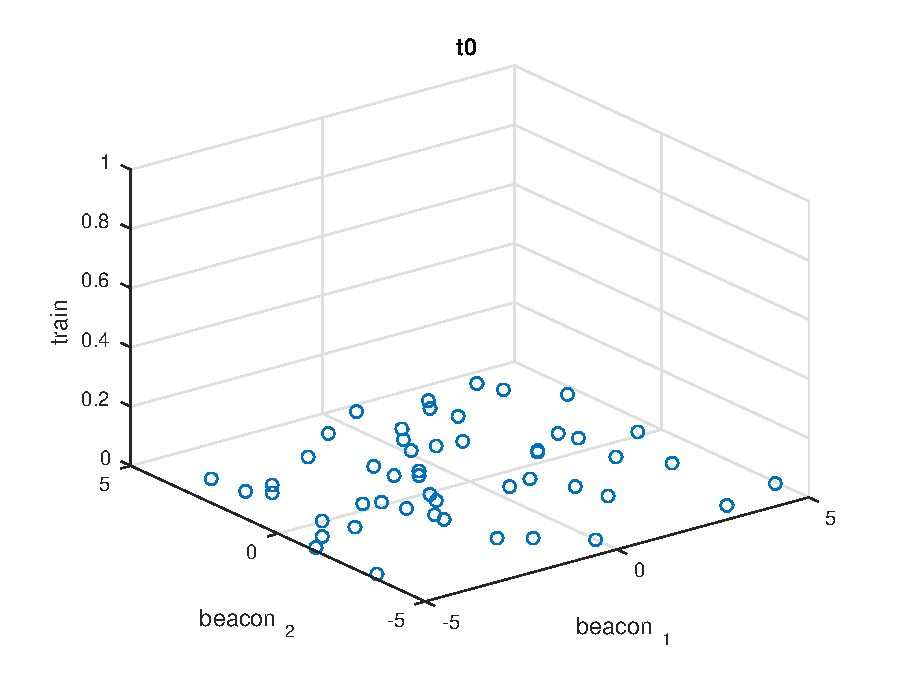
\includegraphics[width=0.8\linewidth]{figures/t0.eps}
	\caption{Particles at t0}
	\label{t0}
\end{figure}

\subsection{$t_1$}

All particles in the plane $(beacon\_1,beacon\_2)$ spread uniformly, $train=10$ for all particles with small variance.


\begin{figure}[H]
	\centering
	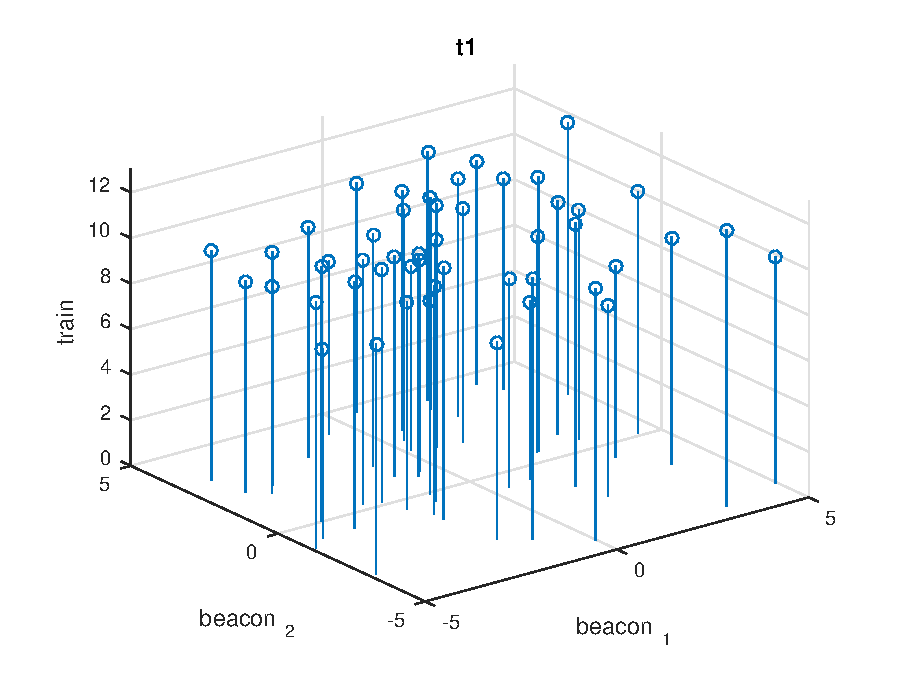
\includegraphics[width=0.8\linewidth]{figures/t1.eps}
	\caption{Particles at t1}
	\label{t1}
\end{figure}


\subsection{$t_2$}

All particles uniformly distributed along a line parallel to $beacon_2$ axis, $beacon_1 = 25$ with medium  variance (larger than variance in $train$ axis), $train=10$ for all particles with same variance as in $t_1$.


\begin{figure}[H]
	\centering
	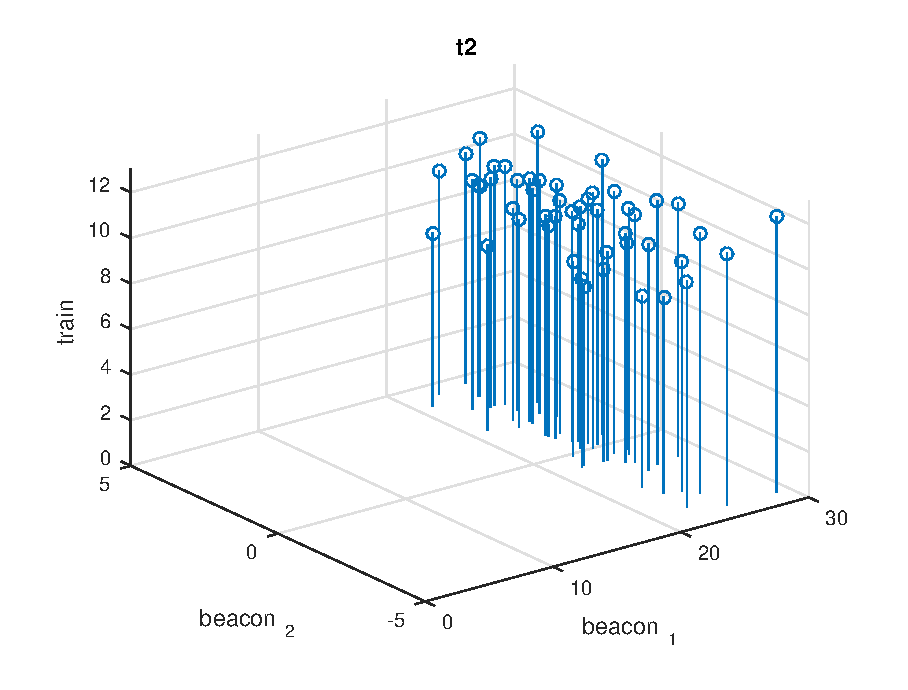
\includegraphics[width=0.8\linewidth]{figures/t2.eps}
	\caption{Particles at t2}
	\label{t2}
\end{figure}


\subsection{$t_3$}

$beacon_2 = 5$ with medium variance, $beacon_1 = 25$ with medium  variance (same as in $t_2$), $train=10$ for all particles with same variance as in $t_1$ and in $t_2$.


\begin{figure}[H]
	\centering
	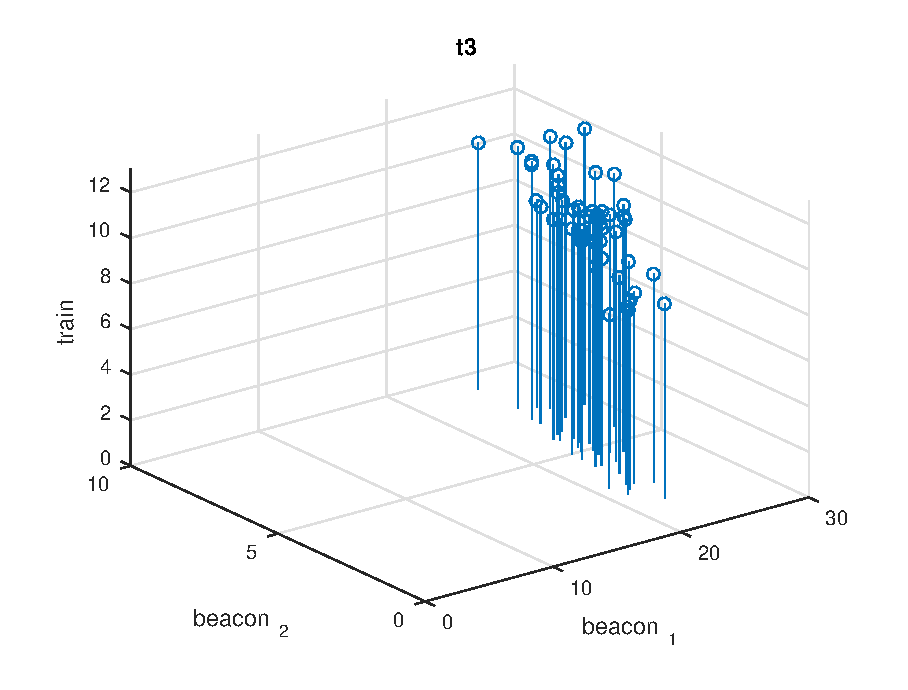
\includegraphics[width=0.8\linewidth]{figures/t3.eps}
	\caption{Particles at t3}
	\label{t3}
\end{figure}


\subsection{$t_4$}

$beacon_2 = 5$ with medium variance, $beacon_1 = 25$ with medium  variance, $train=30$ with larger variance than before.



\begin{figure}[H]
	\centering
	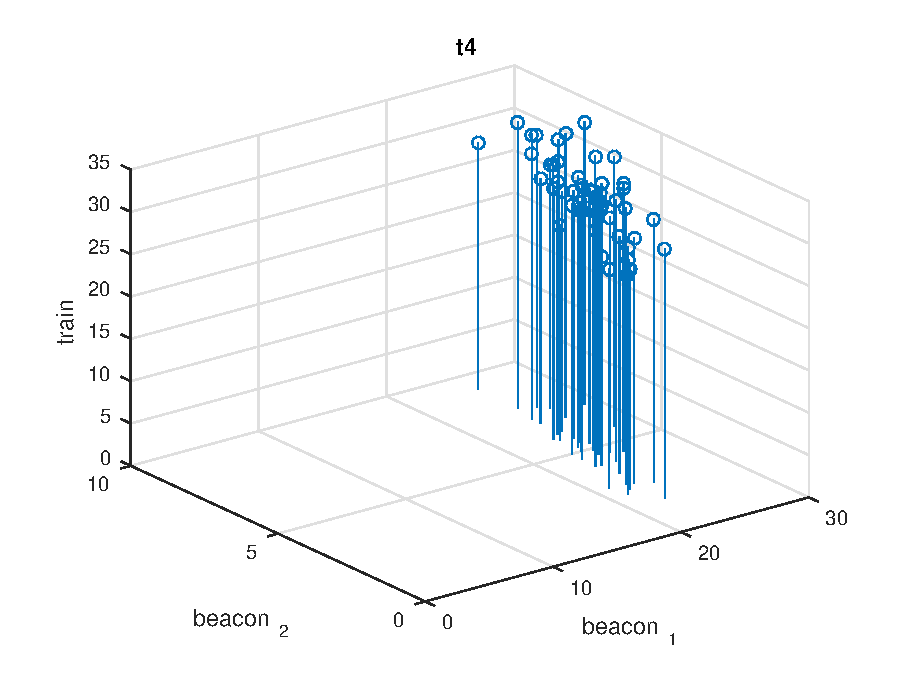
\includegraphics[width=0.8\linewidth]{figures/t4.eps}
	\caption{Particles at t4}
	\label{t4}
\end{figure}



\end{document}


